\section{まえがき}

\begin{figure}[b]
    \begin{center}
        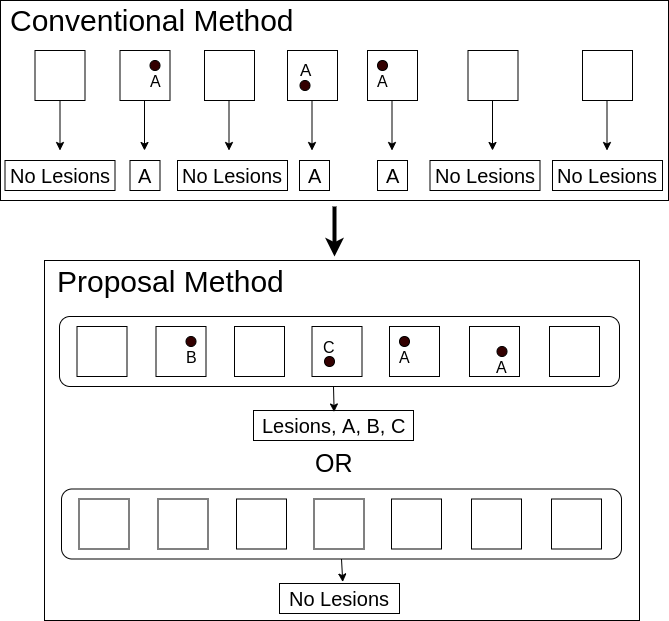
\includegraphics[width=80mm]{./fig/0.png}
        \caption{Overview}
        \label{fig:overview}
    \end{center}
\end{figure}

現在機械学習の分野において深層学習による画像処理\cite{CNN,AlexNet,VGG,ResNet}、系列データ処理\cite{RNN,GRU,LSTM,Transformer}が高い精度を記録している。このため文字や画像や音声などの認識\cite{DL_LVCSR,ImageNet}や生成\cite{GAN,VAE}、翻訳\cite{Transformer,Seq2Seq,effective_attention}や検索\cite{anxious_learning}といった自然言語処理に幅広く用いられるようになっている。また化合物の性質予測\cite{Chemistry1,Chemistry2}やゲノム構造の解析\cite{Genomics}、株価の予測\cite{stock_prediction}のように、生物学や化学や経済学などの情報工学分野を超えた様々な分野においても用いられてきている。

この流れの中で医学分野においても様々な用途で深層学習が用いられてきている。例としては皮膚画像による皮膚ガンメラノーマの判定\cite{skin_cancer_melanoma}や放射線画像による深層学習解析\cite{radiology}などがあげられる。

他にも医学分野において深層学習を用いた自動化によって診断の精度向上や作業の効率化が期待できる用途がある。その中でも内視鏡画像の解析が挙げられる。既存研究には、内視鏡画像による胃癌判定\cite{stomach_cancer}や食道癌\cite{esophageal_cancer}の判定がある。これらの研究は内視鏡画像を一枚ずつラベル付けして学習したもので、内視鏡検査における画像全体を学習していない。このためより効果的な用途として内視鏡画像からの簡易カルテの生成が挙げられる。現在簡易カルテの生成は人手によって行われており、各患者ごとに数分の時間がかかっている。さらに大量の2重チェックを行う必要がある。したがって医師の貴重な時間の多くを簡易カルテ作成に費やさなければならないという大きな問題があった。
これらの作業が自動化されることによる医師の負担削減が大きく期待できる。
また病変見落としが医師によっては2割以上といったデータ\cite{medical_problem2}もある。自動化により精度の高い予測が可能になると、病変の見落としなども減らすことが可能になる。

しかしながら深層学習を医学分野に用いることに関していくつかの問題がある。一つ目は倫理的な問題である。医療における診断という大きな責任を伴う判断において、深層学習のような機械学習モデルを用いることには責任の所在がなくなるという課題がある。現在の深層学習モデルはブラックボックスであり、判断の根拠が不明となっている。このため医療分野における責任ある判断をまかせることにはまだ至っていない。二つ目はプライバシーの問題である。患者の診断データや内視鏡画像は重要度の非常に高いプライバシーデータであり、実際の推論システムにおいて患者のデータが特定可能な形で出力されてしまうことを必ず避けなければならない。

本研究では簡易カルテという精密検査や診断の確定がなされる前の作業における支援システムとして導入するため、最終的な判断の責任は医師にある。また学習データの作成では、簡易カルテから学習データのマルチラベルを作成するに当たって、質的診断の項目を自動で収集してマルチラベル化するため、プライバシー情報が完全に学習データに含まれない。学習においても、内視鏡画像とマルチラベルデータのみを深層学習モデルに通した。

既存研究では各患者に対して数十枚ある内視鏡画像すべてに手動で病名情報をラベリングしている。したがって深層学習を用いるためには数十万の学習データを用意する必要があるために膨大な時間がかかっている。全ての画像においてラベリングをした教師あり学習であるために高い精度を記録しているが、推論時も各画像単位で行われるため、画像を用いた診断として用いることはできるが簡易カルテの作成の自動化には至っていない。このため本研究では医師が作成した簡易カルテに対して自然言語処理を行い、教師データとしてマルチラベルを作成した。このマルチラベルデータは二つの部分から構成されている。一番目のラベルは内視鏡画像の中に病変があるか否かを示す値が格納されており、二番目以降は頻出病名に対応した複数のラベルが並んでいる。マルチラベルデータは簡易カルテの病名情報を要約したものとして用いることができる。内視鏡画像とマルチラベルデータの関係性を直接学習させることによって、学習データの作成と学習全ての工程を自動化することに成功した。

学習手法に関しては、大きく分けて二つの手法で実験した。一つ目の手法は各患者における数十枚の画像をそれぞれ一枚ずつ入力し、出力をマルチラベルから損失を計算し、モデルを学習するものである。二つ目の手法では各患者の全ての画像を3次元データとして用いてモデルを学習した。

本論文では作成した学習データを二つの手法においてそれぞれ複数の深層学習モデルで学習と推論を行い、結果を比較した。

以下、第2章で関連研究について述べ、第3章で提案手法について、第4章で評価実験、第5章で考察、第6章で結論を述べる。
